%%%%%%%%%%%%%%%%%%%%%%%%%%%%%%%%%%%%%%%%%
% Journal Article
% LaTeX Template
% Version 1.3 (9/9/13)
%
% This template has been downloaded from:
% http://www.LaTeXTemplates.com
%
% Original author:
% Frits Wenneker (http://www.howtotex.com)
%
% License:
% CC BY-NC-SA 3.0 (http://creativecommons.org/licenses/by-nc-sa/3.0/)
%
%%%%%%%%%%%%%%%%%%%%%%%%%%%%%%%%%%%%%%%%%

%----------------------------------------------------------------------------------------
%	PACKAGES AND OTHER DOCUMENT CONFIGURATIONS
%----------------------------------------------------------------------------------------

\documentclass[twocolumn]{article}

\usepackage{lipsum} % Package to generate dummy text throughout this template
\usepackage[utf8x]{inputenc}
\usepackage[T1]{fontenc}
\PrerenderUnicode{áéíóúñ}
%\usepackage[spanish]{babel}
%\usepackage{t1enc}
\usepackage[english]{babel}
\usepackage{graphicx}
\usepackage{sidecap}
\usepackage{amssymb,amsmath}
\usepackage{mathtools}
\usepackage{amsmath}
\usepackage{mathrsfs}
\usepackage{float} 
\usepackage[sc]{mathpazo} % Use the Palatino font
\usepackage[T1]{fontenc} % Use 8-bit encoding that has 256 glyphs
\linespread{1.05} % Line spacing - Palatino needs more space between lines
\usepackage{microtype} % Slightly tweak font spacing for aesthetics
\usepackage{url}
\usepackage[hmarginratio=1:1,top=15mm,columnsep=15pt,left=15mm]{geometry} % Document margins
\usepackage{multicol} % Used for the two-column layout of the document
\usepackage[hang, small,labelfont=bf,up,textfont=it,up]{caption} % Custom captions under/above floats in tables or figures
\usepackage{booktabs} % Horizontal rules in tables
\usepackage{float} % Required for tables and figures in the multi-column environment - they need to be placed in specific locations with the [H] (e.g. \begin{table}[H])
\usepackage{hyperref} % For hyperlinks in the PDF
\usepackage{caption}
\usepackage{lettrine} % The lettrine is the first enlarged letter at the beginning of the text
\usepackage{paralist} % Used for the compactitem environment which makes bullet points with less space between them
\def\textsubscript#1{\ensuremath{_{\mbox{\textscale{.6}{#1}}}}}
\usepackage{abstract} % Allows abstract customization
\renewcommand{\abstractnamefont}{\normalfont\bfseries} % Set the "Abstract" text to bold
\renewcommand{\abstracttextfont}{\normalfont\small\itshape} % Set the abstract itself to small italic text
\usepackage{titlesec} % Allows customization of titles
\graphicspath{ {pics/} }
\titleformat{\section}[block]{\large\scshape\centering}{\thesection.}{1em}{} % Change the look of the section titles
\titleformat{\subsection}[block]{\large}{\thesubsection.}{1em}{} % Change the look of the section titles
\renewcommand{\labelitemi}{$\bullet$}
\renewcommand{\labelitemii}{$\cdot$}
\renewcommand{\labelitemiii}{$\diamond$}
\renewcommand{\labelitemiv}{$\ast$}


%\usepackage{fancyhdr} % Headers and footers
%\pagestyle{fancy} % All pages have headers and footers
%\fancyhead{} % Blank out the default header
%\fancyfoot{} % Blank out the default footer
%\fancyhead[C]{Metallicity Gradients in ies $\bullet$ December 2015} % Custom header text
%\fancyfoot[RO,LE]{\thepage} % Custom footer text

%----------------------------------------------------------------------------------------
%	TITLE SECTION
%----------------------------------------------------------------------------------------

\title{\vspace{-20mm}\fontsize{16pt}{10pt}\selectfont\textbf{Continuum determination}} % Article title

\author{
%\large
\textsc{Lynge R. B. Lauritsen} \\
\normalsize University of Copenhagen \\ % Your institution
\date{March 2018}
\vspace{-9mm}
}
%----------------------------------------------------------------------------------------

\usepackage{amsmath}
\begin{document}
\begin{multicols}{1}
\maketitle % Insert title
\end{multicols}{}

%\thispagestyle{fancy} % All pages have headers and footers

%----------------------------------------------------------------------------------------
%	ABSTRACT
%----------------------------------------------------------------------------------------

%\begin{abstract}

%\noindent ABSTRACT

%\end{abstract}

%----------------------------------------------------------------------------------------
%	ARTICLE CONTENTS
%----------------------------------------------------------------------------------------
%\begin{multicols}{2} % Two-column layout throughout the main article text


\section{Finding Continuum}
In this section the process utilised in determining the used continuum destribution of the observed quasar data is described. The method used was found through a combination of reading relevant literature and implementation of numerical MCMC algorithm. At no point in this endeavor has the aim been to find the absolute Continuum Light Curve (CLC). The objectively correct CLC is of no real importance in the investigation, and therefore would cause unnecessary time to pursue. The difficulty in determining the absolute CLC is in the lack of knowledge of the actual band dependent transfer function of the observed Light Curves (LC). Additionally the interest in the project is the timelag between the observable bands, and as such the relative transfer functions as opposed the the absolute transfer functions. \\
This section will be focused upon describing the methods used and the reasons behind the decisions taken.\\

\subsection{Original Data Material and Kelly manipulations}
The CLC is found based upon the observed light curves of the K-band. The REM data is observed in the KHJgriz bands. The REM data is uneven in the sampling and subject to several observation gaps of a 50 - 100 day period. Due to this sampling it has proved of interest to attempt to simulate the Observed Light Curves (OLC) across the observational gaps. These has been filled through the use of the Kelly Function (Kelly et al. 2009). The Kelly Function is not actually a function as much as a way of approximating the next point of the LC based upon the overall distribution of observed values. It is given by \emph{equation \ref{eq:Kelly2009}},

\begin{equation}
dX(t) = -\frac{1}{\tau}X(t)dt + \sigma\sqrt{dt}\epsilon(t) + bdt
\label{eq:Kelly2009}
\end{equation}
with \emph{b} being the observed mean value of the OLC and $\tau$ is the relaxation time. The Kelly approach introduces a bias designed to pull the LC towards the mean. To counter this offset the Kelly approach has been applied in both directions of the LC and the mean of the two functions is the accepted value. The $\epsilon$ is a white noise process with mean zero and standard deviation of one. This is examplified in \emph{figure \ref{fig:NGC3783K-Kelly}}

\begin{figure}[htp!]
\centering
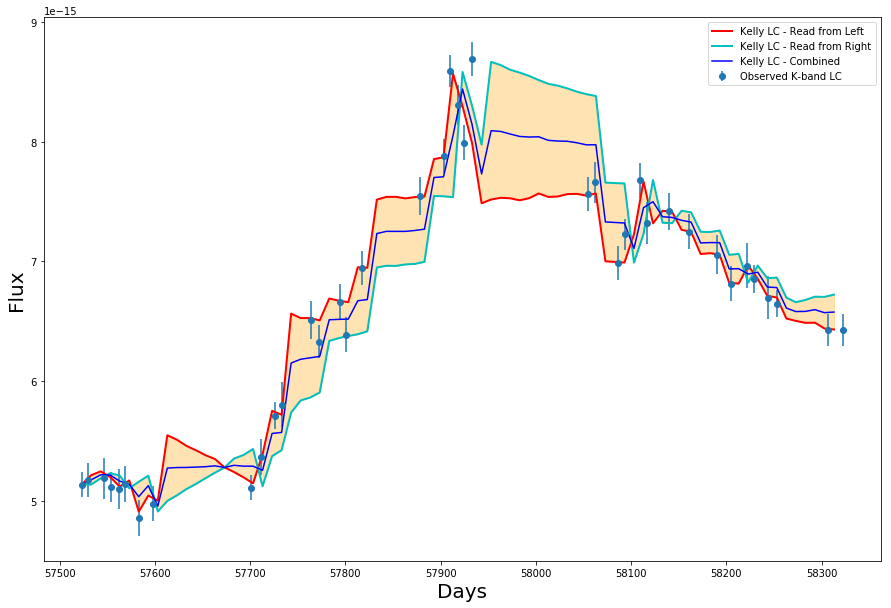
\includegraphics[width=1\linewidth]{/home/lynge/MasterP/Figure/NGC3783K-Kelly.png}\\
\caption{The Kelly function applied to the NGC3783 K-band spectrum.}
\label{fig:NGC3783K-Kelly}
\end{figure}

The weakness of the Kelly method becomes clear in the second interval of missing data points (around 57800 - 57900 MJD). The Kelly Function breaks down in this area, it may be possible to adjust this somewhat by introducing a dependence of time from the points of observation that the estimate is based upon. This however is not the focus at this time. \\
\\
\subsection{Transfer Functions}
In order to determine the CLC one must have an understanding of how the LC behaves from the Quasar to the observation. If one were to determine the exact Transfer Function at all times, it would then be possible to determine the exact CLC. However the transfer function is an unknown quantity and as the OLC is the result of the transfer function and the OLC (\emph{equation \ref{eq:OLC}}) (Andreas Skielboe 2016)
\begin{equation}
F_l(t,\lambda) = \int_{-\infty}^{\infty}\Psi(\tau,\lambda)F_C(t-\tau)d\tau
\label{eq:OLC}
\end{equation}
it is impossible to accurately determine the CLC. However this project is not concerned with the accurate CLC, it is however interested in the relative difference between the Transfer Functions. It is therefore decided to assume a Transfer Function for the K-band data. Using this arbitrary function, \emph{equation \ref{eq:OLC}} and an MCMC algorithm a possible CLC is determined. This possible CLC can then be utilised in compound with the OLC for the renmaining observed bands and \emph{equation \ref{eq:OLC}} to determine the relative differences and hence the timelag between the Transfer Functions. \\
For arbitrary Transfer Function a log-normal is chosen (\emph{equation \ref{eq:TF}})
\begin{equation}
f(x) = \frac{1}{x\sigma\sqrt{2\pi}}e^{-\frac{(ln(x))^2}{2\sigma^2}}
\label{eq:TF}
\end{equation}

\subsection{Power Spectral Density}
OLC from AGN's has distinct Power Spectral Densities (PSD's). This detail is used to determine whether the outcome from the MCMC algorithm is in fact a CLC, or just one of infinitely many possible solutions that exists to the numerical solving of \emph{equation \ref{eq:TF}}. The PSD slope is generally in the vicinity -2 to -3. The PSD is given by \emph{equation \ref{eq:PSD}} (Uttley et al. 2002).
\begin{equation}
P(\nu) = \frac{2T}{\mu^2N^2}|F_N(\nu)|^2
\label{eq:PSD}
\end{equation}
with $|F_N(\nu)|^2$ given by \emph{equation \ref{eq:F_N}}
\begin{equation}
|F_N(\nu)|^2 = [\sum_{i=1}^{N}f(t_i)cos(2\pi\nu t_i)]^2 + [\sum_{i=1}^{N}f(t_i)sin(2\pi\nu t_i)]^2
\label{eq:F_N}
\end{equation}

\subsection{MCMC algorithm and reasoning}
The CLC is determined through an MCMC type algorithm. An initial guess for the CLC is made and the quality of the fit is made through the use of a variety of factors. 
\begin{enumerate}
\item Determining the residuals squared of the $F_l(t,\lambda)$
\item Determining the double derivative of the CLC
\item Determining the PSD slope of the CLC
\item Producing a Kelly fitting for the CLC
\end{enumerate}
The code then randomly alters the first point on the CLC and item 1 through 4 is redetermined and compared. In the case of a favorable outcome the alteration is saved and the code moves onwards to the following point. The favorability of an outcome is evalueated by a series of parameters. 
\begin{enumerate}
\item Residuals: In all cases the sum of the residuals squared must be less than the previous alteration.
\item Double Derivative: The double derivative is compared to the maximum rate of change of the OLC and is accepted if it is no more than 40 percent larger than the originally observed. This is done to prevent rapid changes to the CLC that would ultimately make for a more stable, but ultimately unphysical solution to the CLC. 40 percent has been chosen as it is felt that despite the OLC becoming somewhat more smooth as a result of the Transfer Function, it would be unlikely to be that prominent. The alternative is the sum of the change in the rate of change of beth adjacent points as well as the altered points decreases overall. This would be accepted as well, pending other factors.
\item PSD slopes: Assuming 1 and 2 holds true, the change can be accepted if the PSD slope is moving closer to the accepted slope, or inside 0.05 of the accepted (so as to allow some freedom of movement of the CLC).
\item Kelly: In the case of 1 holding true, and 2 follows the path of the set of double derivatives overall decreasing there will be a statistical possibility of 5 percent of a change being accepted IF the Kelly function provides an overall better fit and the PSD slope is no more than 0.3 out. This is done primarily to utilise the Kelly function as a method of approximating LC's and hence allowing for the use of this additional resource in providing a more physical fitting, as well as counterbalancing the possibility of the CLC becoming stable in an unstable equilibrium position due to the other limitations.
\end{enumerate}
It is being experimented upon with both one moving point as well as three. 




%----------------------------------------------------------------------------------------
%	REFERENCE LIST
%----------------------------------------------------------------------------------------
\newpage
[1] Kelly et al. 2009, APJ698:895-910 
[2] Kelly et al. 2009, arXiv:0903.5315v1 
[3] A. Skielboe 2016, Thesis 
[4] Uttley et al. 2002 Mon. Not. R. Astron. Soc. 332,231-250

%\end{multicols}
\end{document}
